\documentclass[12]{beamer}
\usepackage[utf8]{inputenc}
%\usepackage[T1]{fontenc}
\usepackage{lmodern}
\usepackage{hyphsubst}%
\usepackage{semtrans}
\usepackage{amsthm}
\usepackage{amsfonts}
\HyphSubstIfExists{ngerman-x-latest}{%
  \HyphSubstLet{ngerman}{ngerman-x-latest}}{}
\HyphSubstIfExists{german-x-latest}{%
  \HyphSubstLet{german}{german-x-latest}}{}
%\usepackage[english,ngerman]{babel}
\usepackage{textcomp}
\usepackage{microtype}
\beamerdefaultoverlayspecification{<+->}

\usetheme{Luebeck}
% Copenhagen
% Dresden
% Hannover
% Luebeck
% Montpellier
% Pittsburgh
% Singapore

\title{Text Generation with LSTM Units}
% \author{Antonio Bozzano Schwedhelm}
\author{By Me}
\date{\today}

\begin{document}
\begin{frame}
\titlepage
\end{frame}
%presentation is about a project i did a couple of months ago

\section{Goals}
\begin{frame}
\frametitle{Goals}
\begin{itemize}
\item<1-> Have fun.
\item<1-> Replicate the results shown in the blog post ``The Unreasonable Effectiveness of Recurrent Neural Networks''.
\end{itemize}
\end{frame}
%really recomend this
%exciting time to be alive
%he used rnns to generate text: text examples -> text generation

%used favourite language: c++
%did it from scratch and made my own matrix class
%looked at what other people were doing way to rarely (seldomly), made stupid mistakes as a result

\section{How Neural Networks Work}
\begin{frame}
\frametitle{How Neural Networks Work}
\begin{itemize}
\item<1-> In general:
$$f_w:\left[-1,1\right]^n\longmapsto\left[-1,1\right]^m$$
% \item<2-> Or:
% $$f_w:\left[0,1\right]^n\longmapsto\left[0,1\right]^m$$
\end{itemize}
\end{frame}
%or a combination

\begin{frame}
\frametitle{How Neural Networks Work}
\begin{itemize}
\item<1-> A neural network consists of layers.
\item<1-> The first layer receives the input, transforms it, and passes it on to the next layer.
\item<1-> Each subsequent layer receives an array from the previous layer, transforms it, and passes it on.
\item<1-> The output of the last layer is the output of the neural network.
\item<2-> Transformation: Multiply the input with a matrix and apply a function to each element of the result.
\end{itemize}
\end{frame}

\begin{frame}
\frametitle{How Neural Networks Work}
\begin{center}
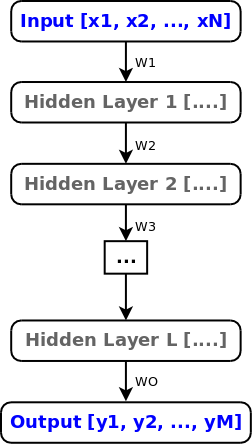
\includegraphics[scale=0.25]{../images/network01.png}
\end{center}
\end{frame}
%do not make a "neuron" class or anythin similar
%you could look at each neuron and each weight individually. In general, this is a bad idea
%ws are the weight matrices. it is the part that learns
%explain what training means

\begin{frame}
\frametitle{How Recurrent Neural Networks Work}
\begin{center}
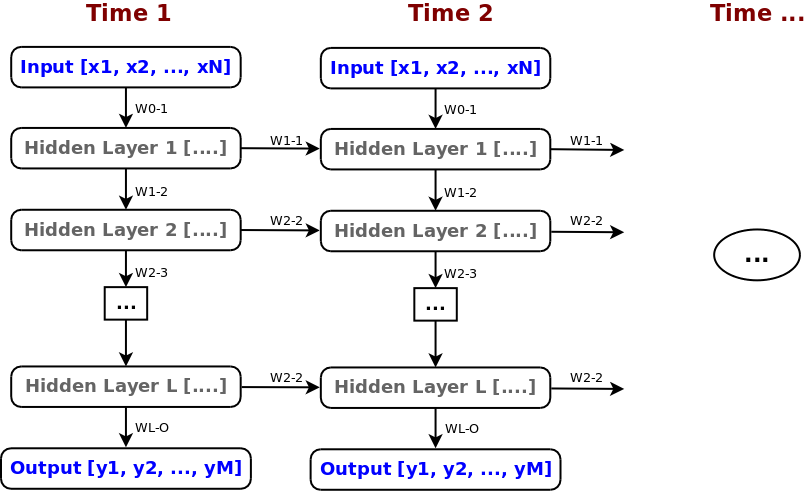
\includegraphics[scale=0.25]{../images/network02.png}
\end{center}
\end{frame}
%and of course, you can do whatever you want here
%layers may or may not be connected in time
%run the nn several times

\section{Constructing a Nueral Network for my Project}
\begin{frame}
\frametitle{The Input}
\begin{itemize}
\item<1-> The neural network is fed characters one at a time.
\item<1-> For this, a mapping from characters to an array of size N is needed.
\item<1-> I used the \textit{one hot} method.
\end{itemize}
\end{frame}

\begin{frame}
\frametitle{One Hot}
\begin{itemize}
\item<1-> If the input is one out of N characters, an array of size N is needed.
\item<1-> Characters are numbered.
\item<1-> Each element is represented by an array of one one an N-1 zeros, where the one is at the position of the characters number.
% \item<1-> Works not just for characters, but any set of distinct elements.
\end{itemize}
\end{frame}

\begin{frame}
\frametitle{One Hot: Example (alphabet)}
\begin{itemize}
\item<1-> $a \longmapsto [1,0,0,0,...,0,0]$
\item<1-> $b \longmapsto [0,1,0,0,...,0,0]$
\item<1-> $c \longmapsto [0,0,1,0,...,0,0]$
\item<1-> $...$
\item<1-> $y \longmapsto [0,0,0,0,...,1,0]$
\item<1-> $z \longmapsto [0,0,0,0,...,0,1]$
\end{itemize}
\end{frame}

\begin{frame}
\frametitle{The output}
\begin{itemize}
\item<1-> The neural network is trained to predict the next character.
\item<1-> It is given the \textit{one hot} representation of the character for training.
\item<1-> After training the output is a probability distribution over the chatacters.
\end{itemize}
\end{frame}
%does not tell you what comes next, but gives you a probability for each characters
%we will coma back to this later

\begin{frame}
\frametitle{What Kinds of Layers are Needed}
\begin{itemize}
\item<1-> I needed three kinds of layers:
\begin{itemize}
\item<1-> Tanh Layers.
\item<1-> LSTM Layers.
\item<1-> Softmax Layers.
\end{itemize}
\end{itemize}
\end{frame}

\begin{frame}
\frametitle{How Does a Tanh Layer Work}
\begin{itemize}
\item<1-> It is a simple mapping: $f_w:\left[-1,1\right]^n\longmapsto\left[-1,1\right]^m$.
\end{itemize}
\end{frame}
%in my case, input can also be (0,1)

\begin{frame}
\frametitle{How Does a LSTM Layer Work}
\begin{itemize}
\item<1-> It is also a mapping: $f_{w,s}:\left[-1,1\right]^n\longmapsto\left[-1,1\right]^m$.
\item<1-> But it has an internal state, meaning that previous runs of the neural network may influence the output.
\end{itemize}
\end{frame}
%wish i could tell you more, cause awesome, but we do not have the time

\begin{frame}
\frametitle{How Does a Softmax Layer Work}
\begin{itemize}
\item<1-> It is a mapping: $f_w:\left[-1,1\right]^n\longmapsto\left[0,1\right]^m$.
\item<1-> Where the output values add up to one, so that the output can be interpreted as a probability distribution.
\end{itemize}
\end{frame}
%again, this is in my case, input can also be (0,1)

\begin{frame}
\frametitle{How Do I Combine them to Generate Text}
\begin{center}
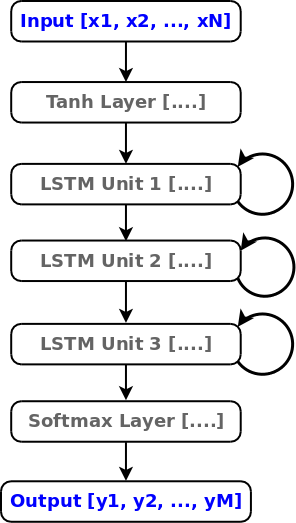
\includegraphics[scale=0.25]{../images/network03.png}
\end{center}
\end{frame}
%didnt experiment a lot, just liked this, and I think it is what was used in the blog
%first tanh is for dimensionality reduction
%adding layers increases the training time linearly: twice as many layers -> twice as much time
%making layers larger, especially LSTM layers, increases time to the power of two: twice as many layers -> four times the time

\section{Gathering Data}
\begin{frame}
\frametitle{Gathering Data}
\begin{itemize}
\item<1-> Gathering enougth data is often a difficult part of deep learning, because a lot of it is needed.
\item<1-> I used two training sets:
\begin{itemize}
\item<1-> CSS files (4.5 GB of them)
\item<1-> A book series (9.3 MB of text)
\end{itemize}
\end{itemize}
\end{frame}

\begin{frame}
\frametitle{Gathering Data: CSS Files}
\begin{itemize}
\item<1-> I built a web crawler that would download every css file it finds (except repeated ones).
\item<1-> Let it run on a NAM computer for a couple of days.
\item<1-> Actually got a complaint for DOS-like behaviour.
\end{itemize}
\end{frame}

\begin{frame}
\frametitle{Gathering Data: CSS Files Made Nice}
\begin{center}
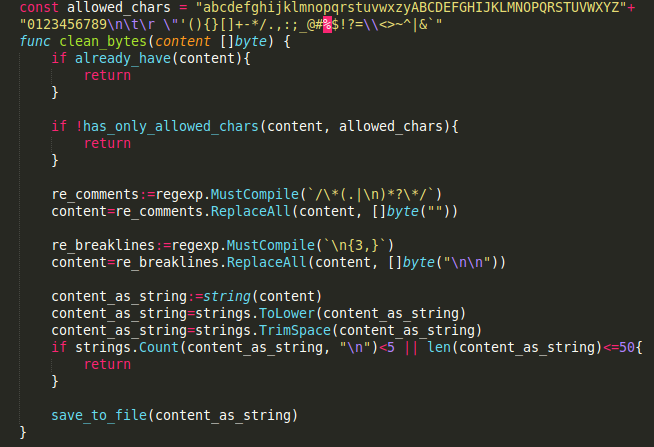
\includegraphics[scale=0.4]{../images/css_filter.png}
\end{center}
\end{frame}

\begin{frame}
\frametitle{Gathering Data: Book Series}
\begin{itemize}
\item<1-> I found the books in text format.
\item<1-> It was an ugly mess translated from scans of the books to text by a computer.
\item<1-> I removed all the garbage I could, transformed it all to lower case, and removed newline characters.
\item<1-> In the end only 46 characters were allowed: \\"! ')(-,.103254769;:?acbedgfihkjmlonqpsrutwvyxz".
\end{itemize}
\end{frame}
%used a python script with mostly regex to find often occurrin errors

% \section{Input/Output Example}
% \begin{frame}
% \frametitle{Input/Output Example}
% \begin{center}
% 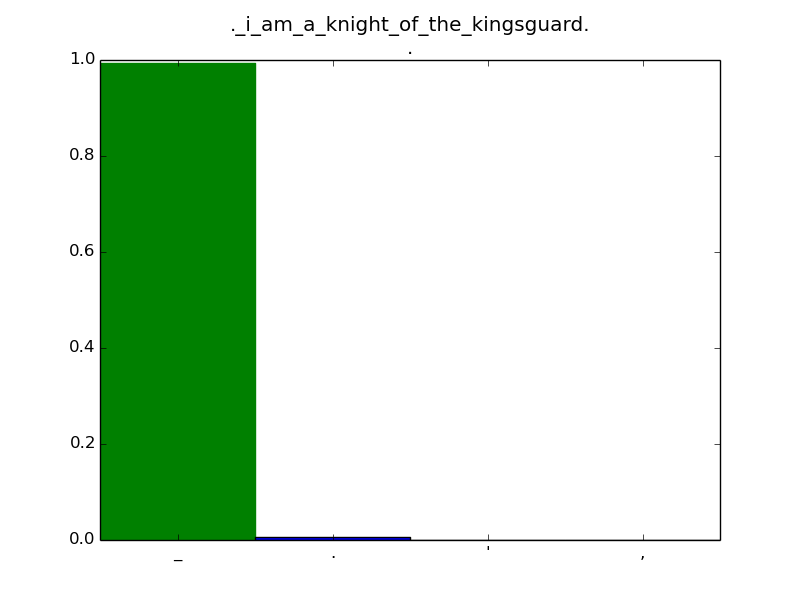
\includegraphics[scale=0.4]{../distplot/00.png}
% \end{center}
% \end{frame}

% \begin{frame}
% \frametitle{Input/Output Example}
% \begin{center}
% 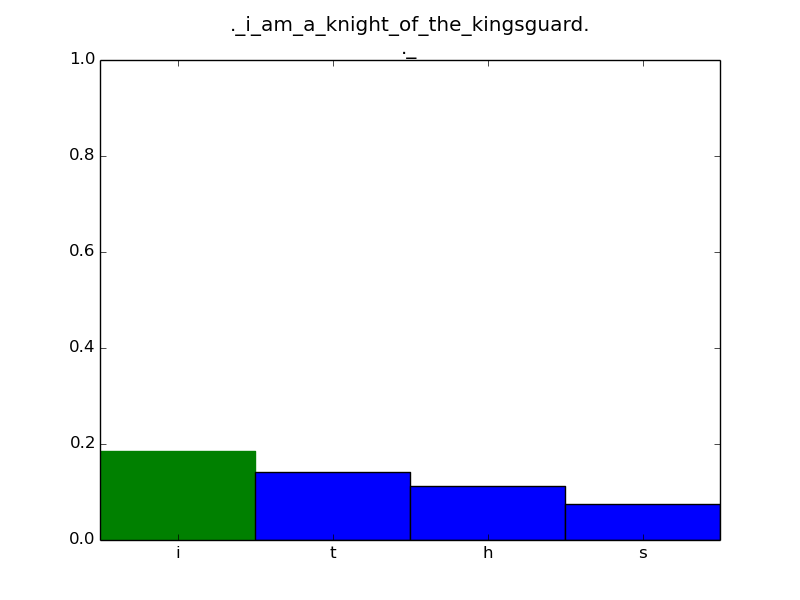
\includegraphics[scale=0.4]{../distplot/01.png}
% \end{center}
% \end{frame}

% \begin{frame}
% \frametitle{Input/Output Example}
% \begin{center}
% 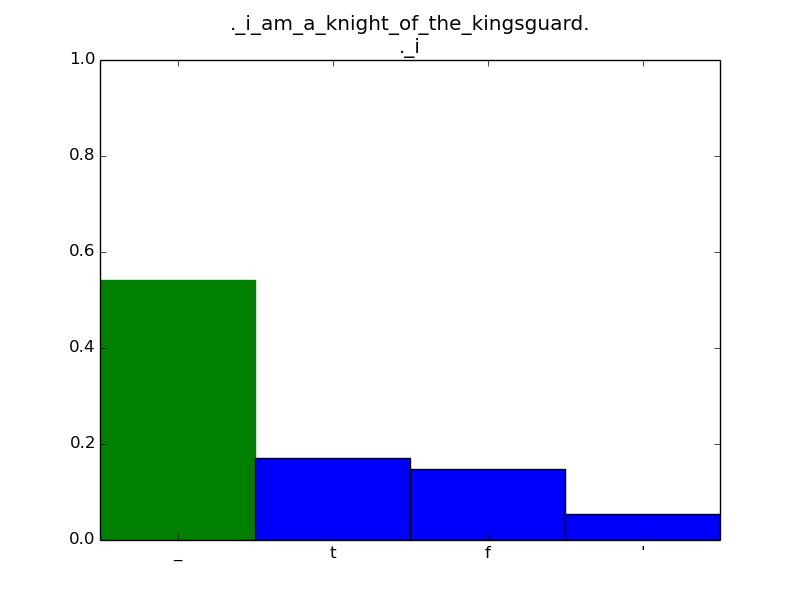
\includegraphics[scale=0.4]{../distplot/02.png}
% \end{center}
% \end{frame}

% \begin{frame}
% \frametitle{Input/Output Example}
% \begin{center}
% 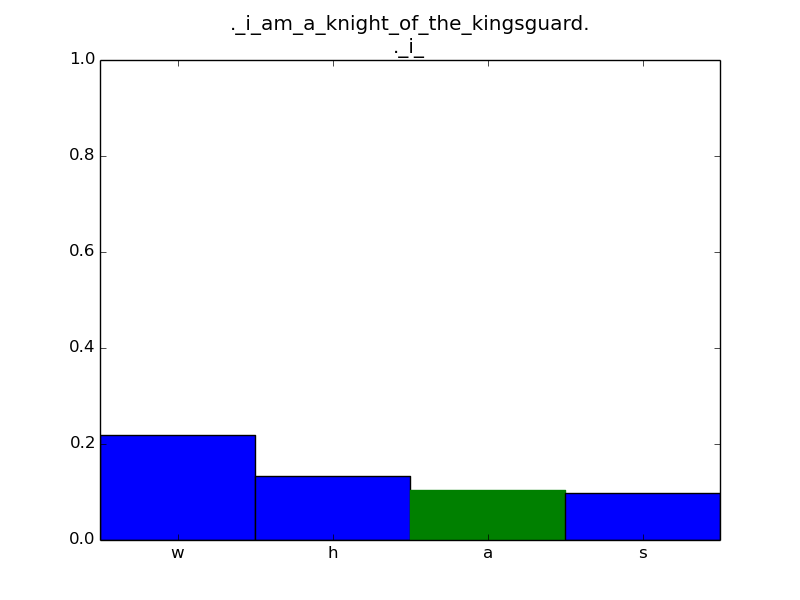
\includegraphics[scale=0.4]{../distplot/03.png}
% \end{center}
% \end{frame}

% \begin{frame}
% \frametitle{Input/Output Example}
% \begin{center}
% 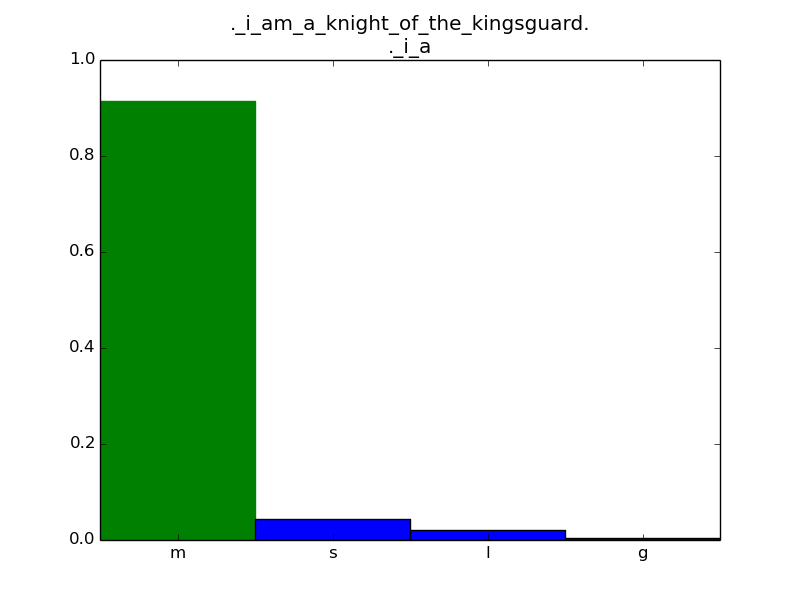
\includegraphics[scale=0.4]{../distplot/04.png}
% \end{center}
% \end{frame}

% \begin{frame}
% \frametitle{Input/Output Example}
% \begin{center}
% 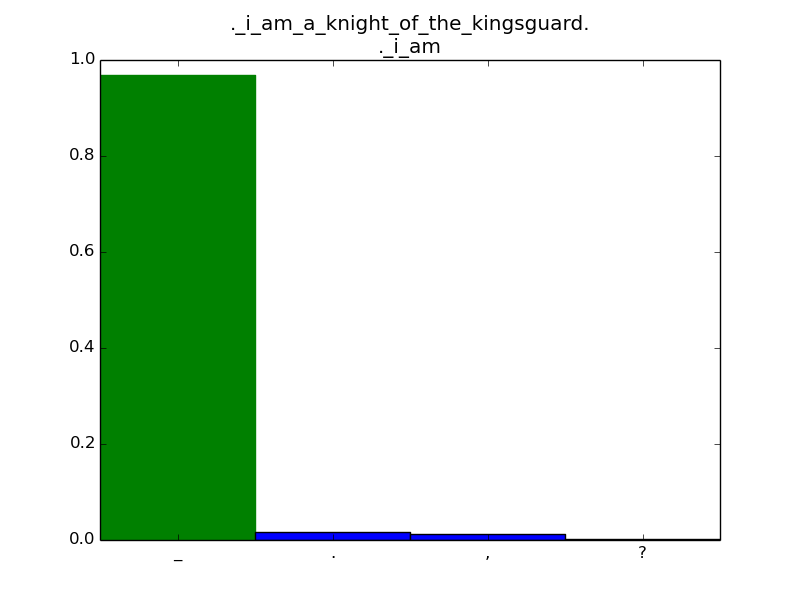
\includegraphics[scale=0.4]{../distplot/05.png}
% \end{center}
% \end{frame}

% \begin{frame}
% \frametitle{Input/Output Example}
% \begin{center}
% 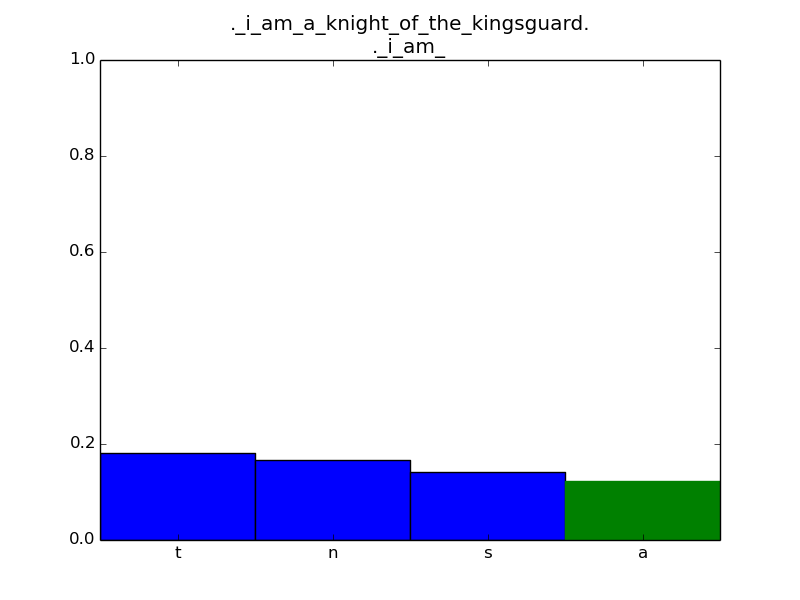
\includegraphics[scale=0.4]{../distplot/06.png}
% \end{center}
% \end{frame}

% \begin{frame}
% \frametitle{Input/Output Example}
% \begin{center}
% 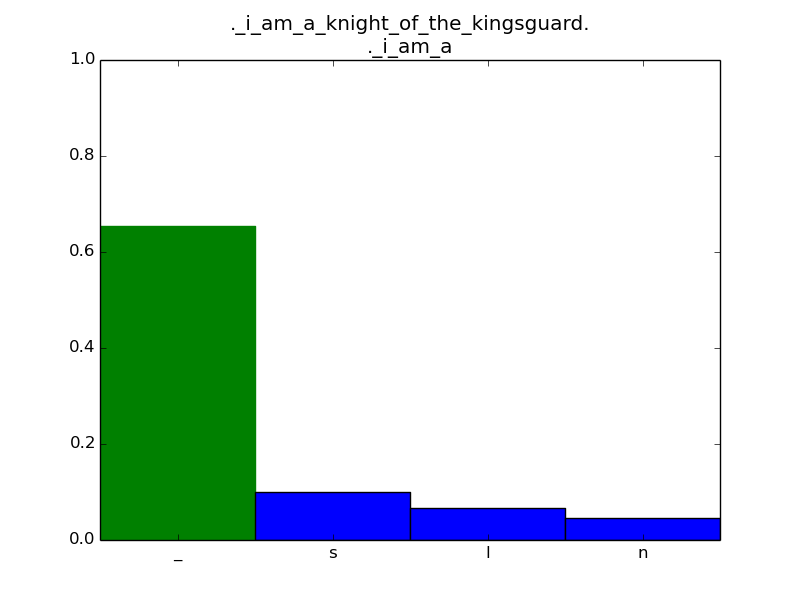
\includegraphics[scale=0.4]{../distplot/07.png}
% \end{center}
% \end{frame}

% \begin{frame}
% \frametitle{Input/Output Example}
% \begin{center}
% 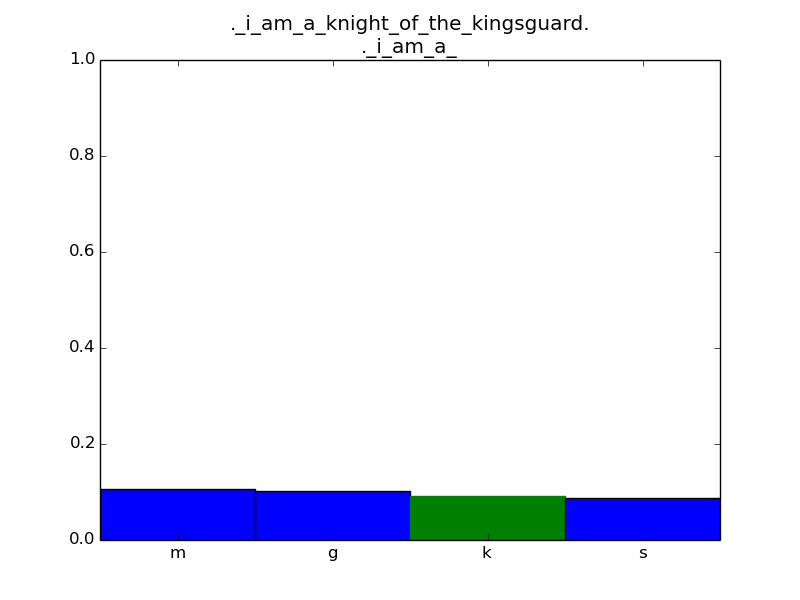
\includegraphics[scale=0.4]{../distplot/08.png}
% \end{center}
% \end{frame}

% \begin{frame}
% \frametitle{Input/Output Example}
% \begin{center}
% 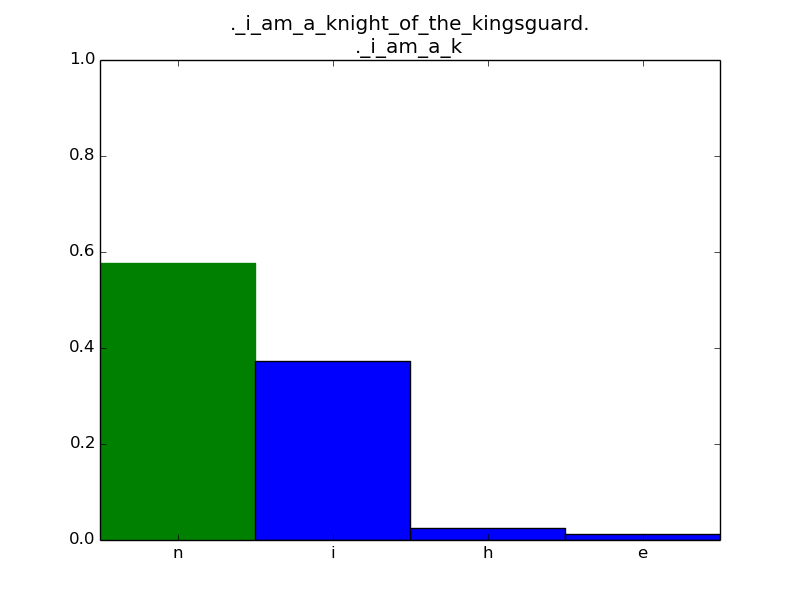
\includegraphics[scale=0.4]{../distplot/09.png}
% \end{center}
% \end{frame}

% \begin{frame}
% \frametitle{Input/Output Example}
% \begin{center}
% 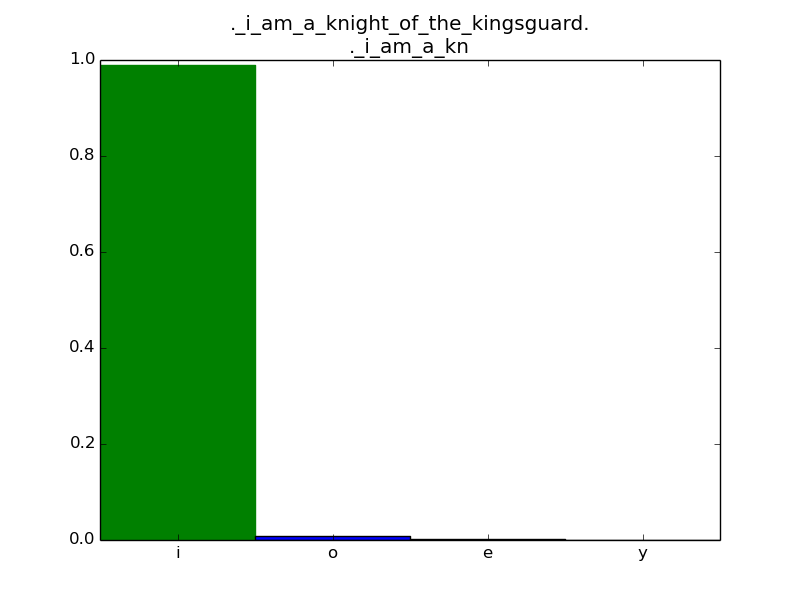
\includegraphics[scale=0.4]{../distplot/10.png}
% \end{center}
% \end{frame}

% \begin{frame}
% \frametitle{Input/Output Example}
% \begin{center}
% 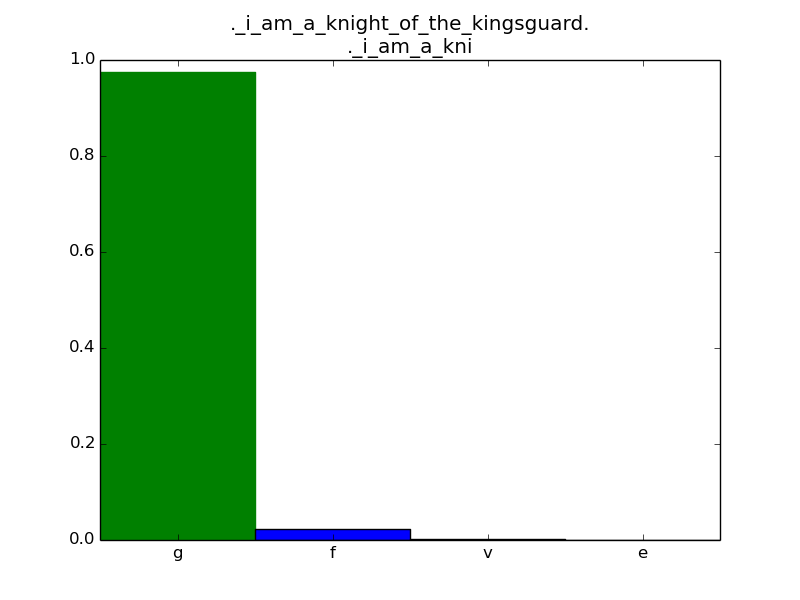
\includegraphics[scale=0.4]{../distplot/11.png}
% \end{center}
% \end{frame}

% \begin{frame}
% \frametitle{Input/Output Example}
% \begin{center}
% 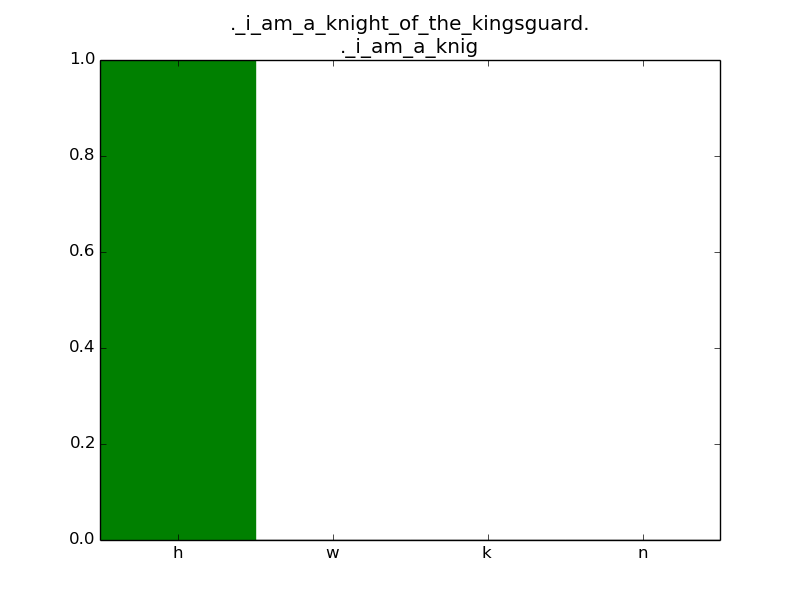
\includegraphics[scale=0.4]{../distplot/12.png}
% \end{center}
% \end{frame}

% \begin{frame}
% \frametitle{Input/Output Example}
% \begin{center}
% 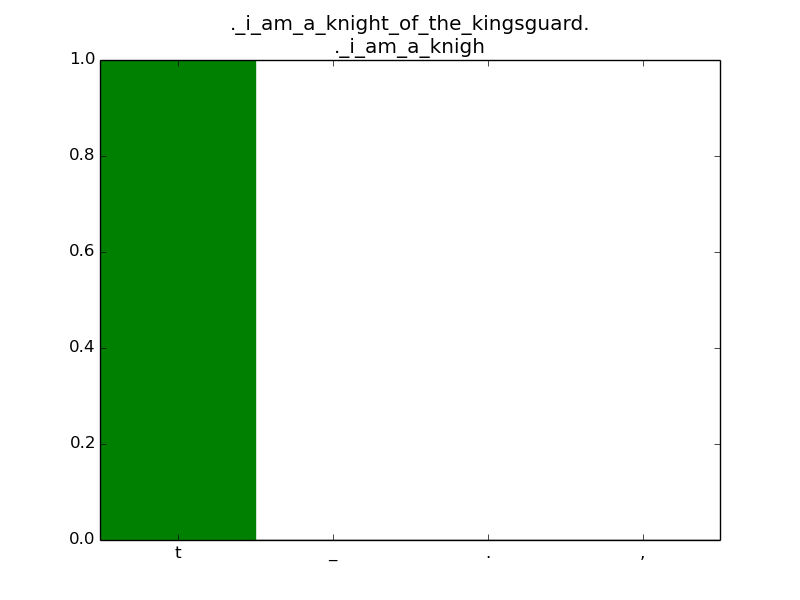
\includegraphics[scale=0.4]{../distplot/13.png}
% \end{center}
% \end{frame}

% \begin{frame}
% \frametitle{Input/Output Example}
% \begin{center}
% 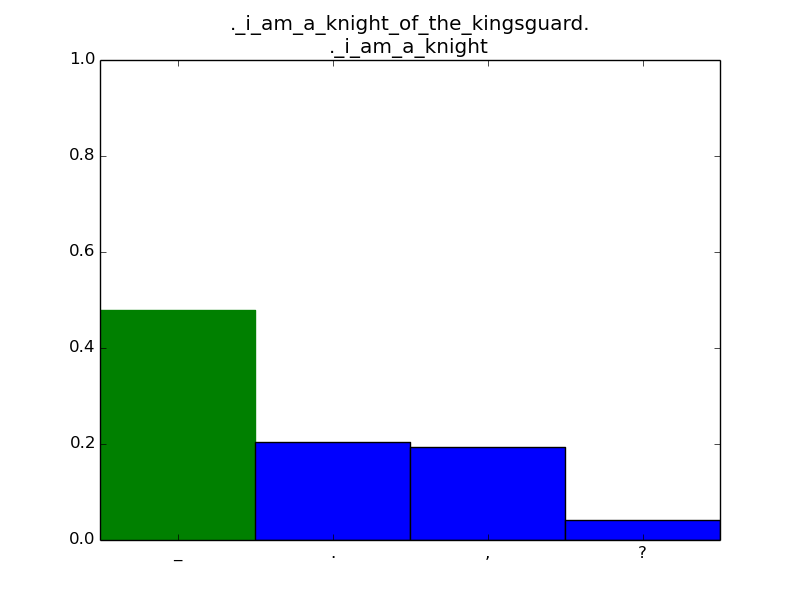
\includegraphics[scale=0.4]{../distplot/14.png}
% \end{center}
% \end{frame}

% \begin{frame}
% \frametitle{Input/Output Example}
% \begin{center}
% 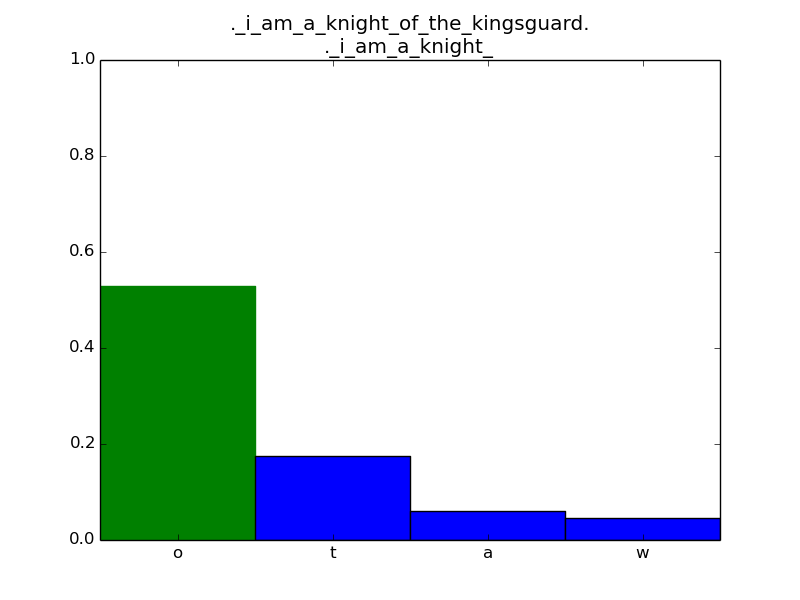
\includegraphics[scale=0.4]{../distplot/15.png}
% \end{center}
% \end{frame}

% \begin{frame}
% \frametitle{Input/Output Example}
% \begin{center}
% 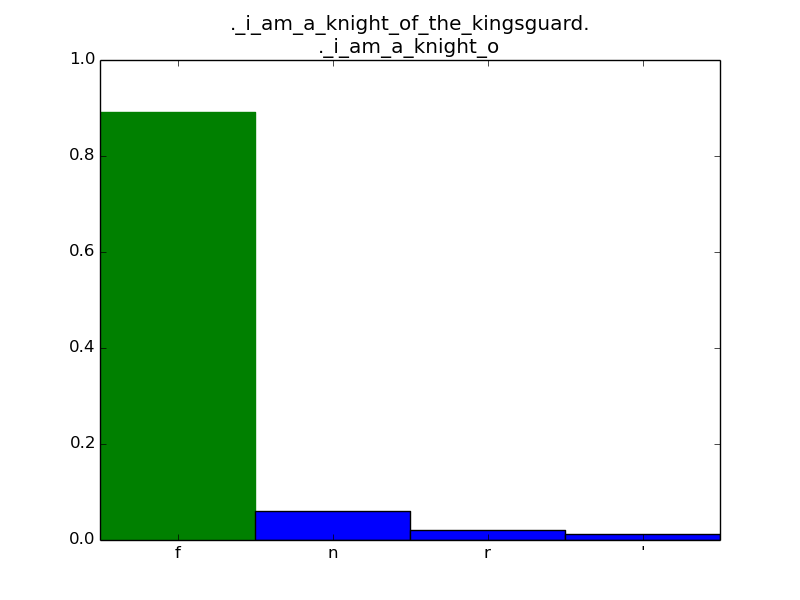
\includegraphics[scale=0.4]{../distplot/16.png}
% \end{center}
% \end{frame}

% \begin{frame}
% \frametitle{Input/Output Example}
% \begin{center}
% 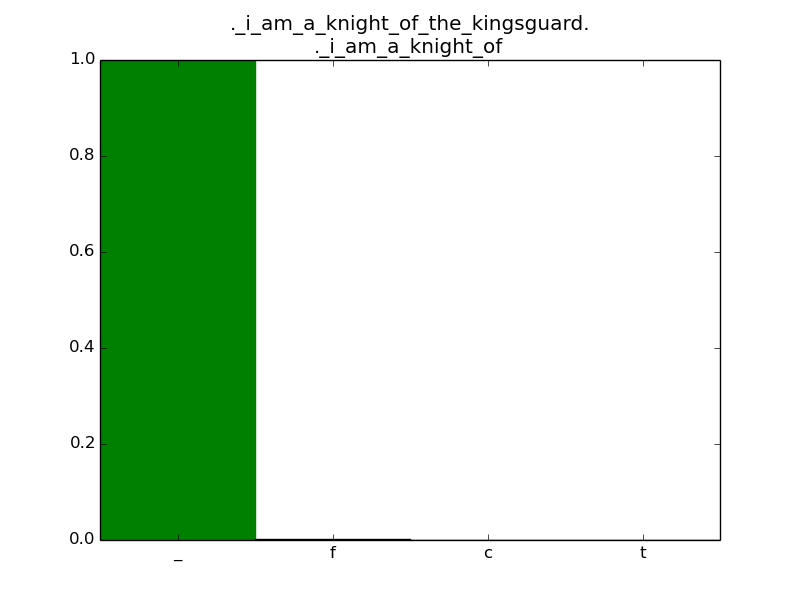
\includegraphics[scale=0.4]{../distplot/17.png}
% \end{center}
% \end{frame}

% \begin{frame}
% \frametitle{Input/Output Example}
% \begin{center}
% 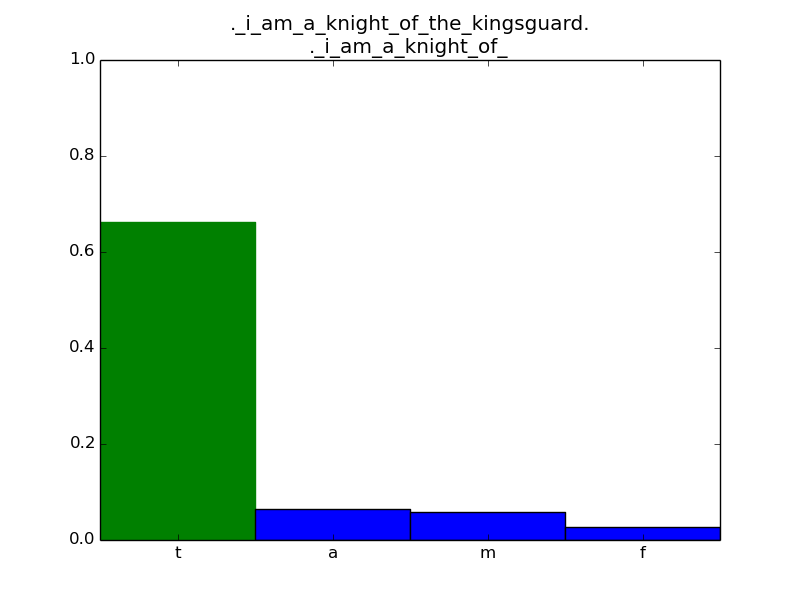
\includegraphics[scale=0.4]{../distplot/18.png}
% \end{center}
% \end{frame}

% \begin{frame}
% \frametitle{Input/Output Example}
% \begin{center}
% 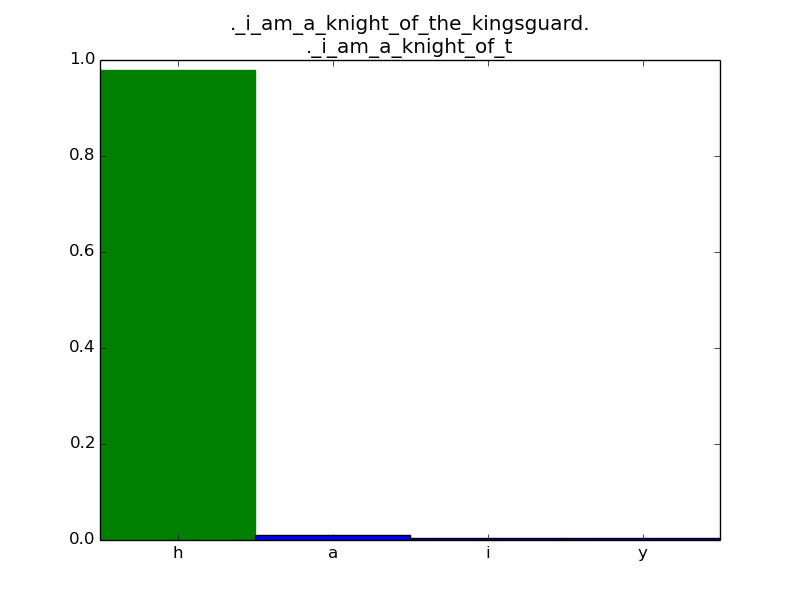
\includegraphics[scale=0.4]{../distplot/19.png}
% \end{center}
% \end{frame}

% \begin{frame}
% \frametitle{Input/Output Example}
% \begin{center}
% 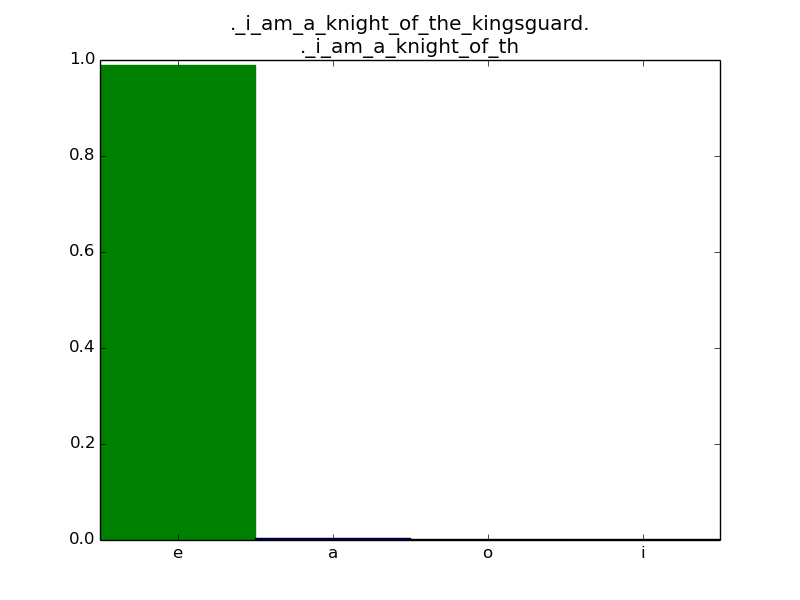
\includegraphics[scale=0.4]{../distplot/20.png}
% \end{center}
% \end{frame}

% \begin{frame}
% \frametitle{Input/Output Example}
% \begin{center}
% 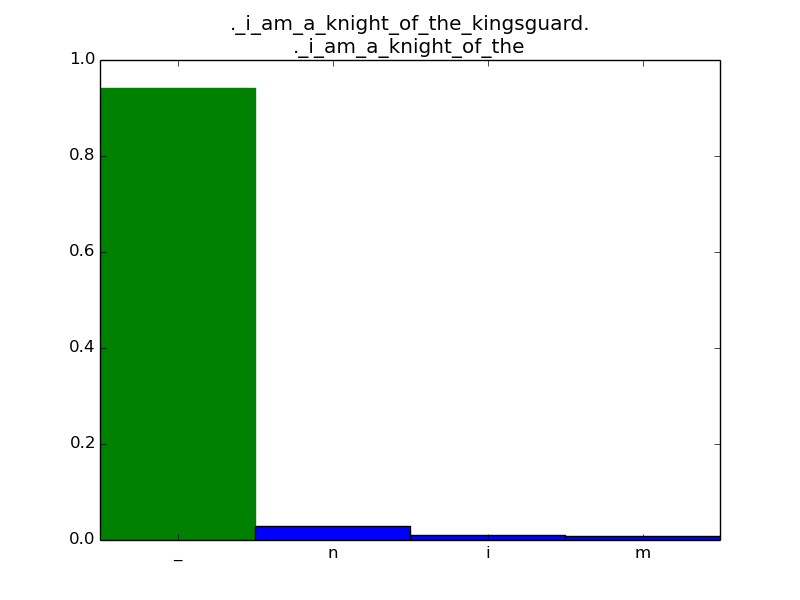
\includegraphics[scale=0.4]{../distplot/21.png}
% \end{center}
% \end{frame}

% \begin{frame}
% \frametitle{Input/Output Example}
% \begin{center}
% 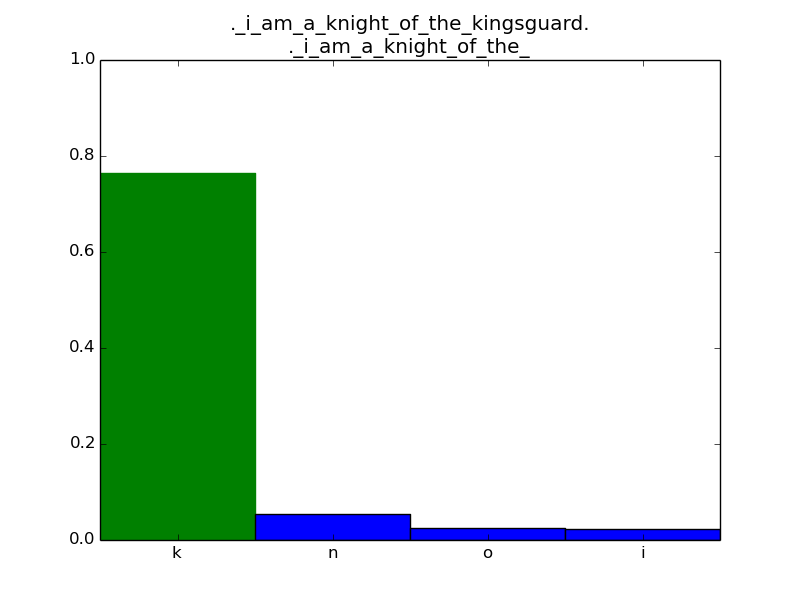
\includegraphics[scale=0.4]{../distplot/22.png}
% \end{center}
% \end{frame}

% \begin{frame}
% \frametitle{Input/Output Example}
% \begin{center}
% 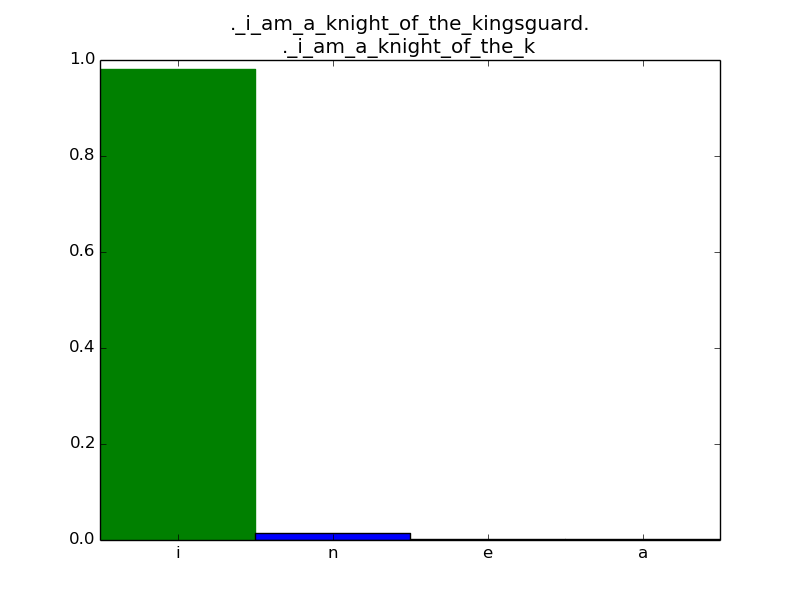
\includegraphics[scale=0.4]{../distplot/23.png}
% \end{center}
% \end{frame}

% \begin{frame}
% \frametitle{Input/Output Example}
% \begin{center}
% 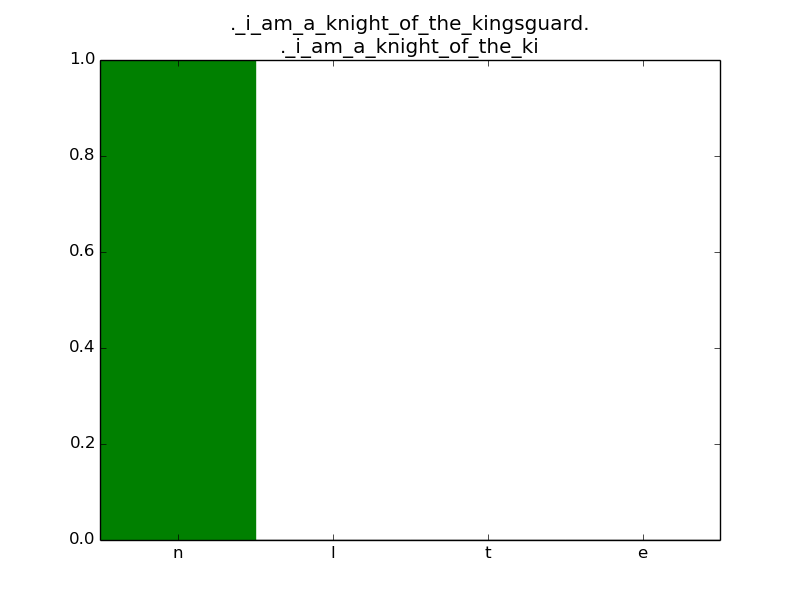
\includegraphics[scale=0.4]{../distplot/24.png}
% \end{center}
% \end{frame}

% \begin{frame}
% \frametitle{Input/Output Example}
% \begin{center}
% 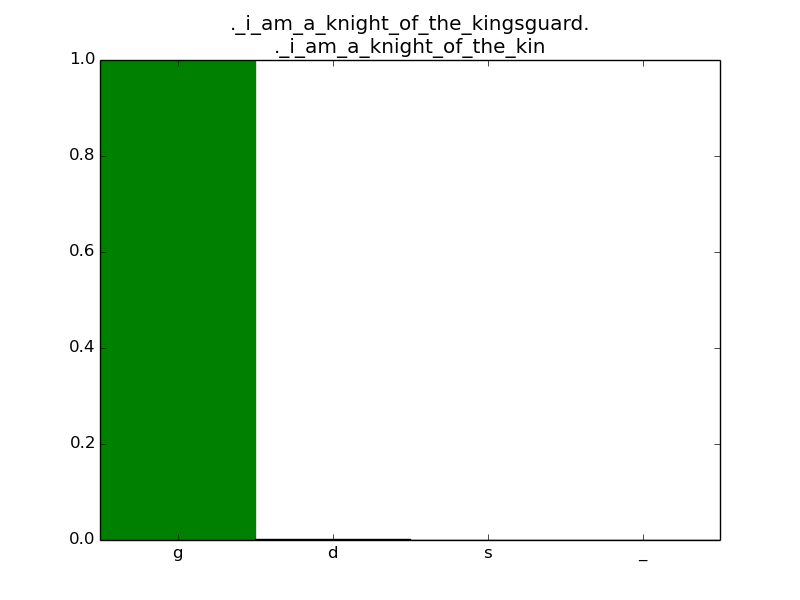
\includegraphics[scale=0.4]{../distplot/25.png}
% \end{center}
% \end{frame}

% \begin{frame}
% \frametitle{Input/Output Example}
% \begin{center}
% 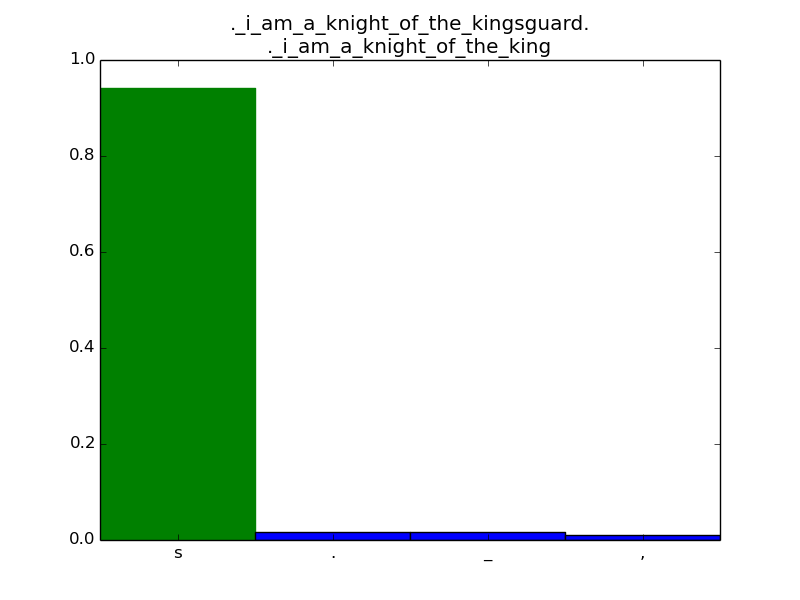
\includegraphics[scale=0.4]{../distplot/26.png}
% \end{center}
% \end{frame}

% \begin{frame}
% \frametitle{Input/Output Example}
% \begin{center}
% 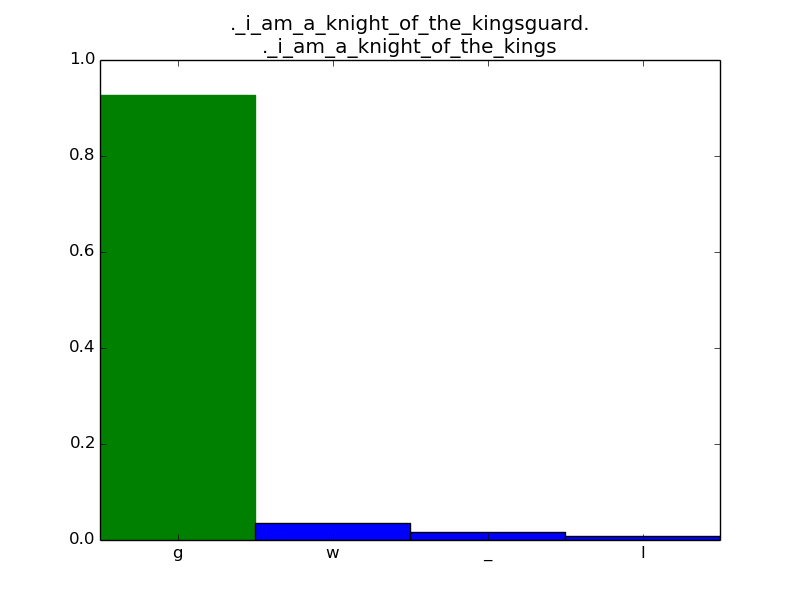
\includegraphics[scale=0.4]{../distplot/27.png}
% \end{center}
% \end{frame}

% \begin{frame}
% \frametitle{Input/Output Example}
% \begin{center}
% 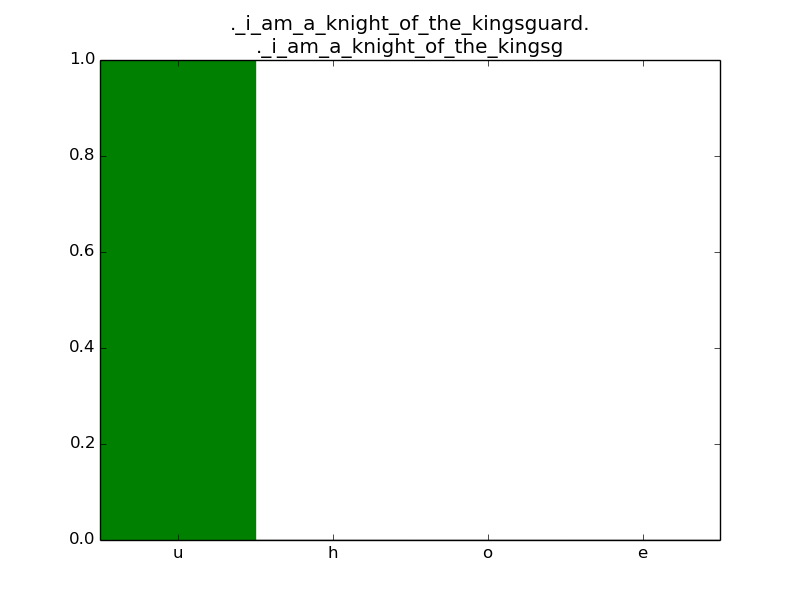
\includegraphics[scale=0.4]{../distplot/28.png}
% \end{center}
% \end{frame}

% \begin{frame}
% \frametitle{Input/Output Example}
% \begin{center}
% 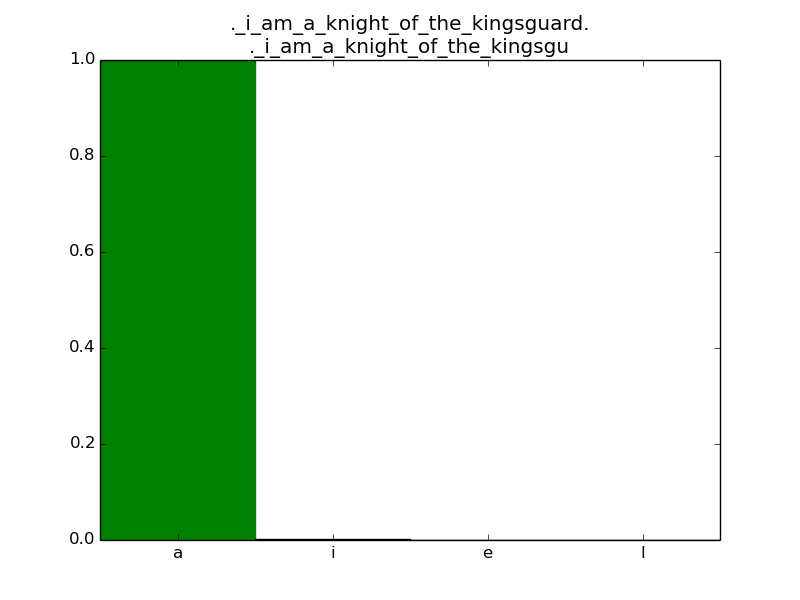
\includegraphics[scale=0.4]{../distplot/29.png}
% \end{center}
% \end{frame}

% \begin{frame}
% \frametitle{Input/Output Example}
% \begin{center}
% 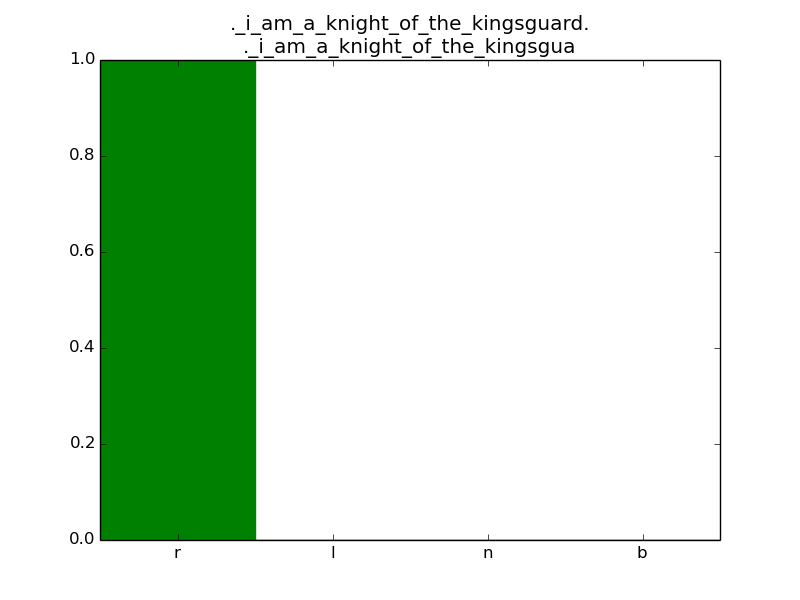
\includegraphics[scale=0.4]{../distplot/30.png}
% \end{center}
% \end{frame}

% \begin{frame}
% \frametitle{Input/Output Example}
% \begin{center}
% 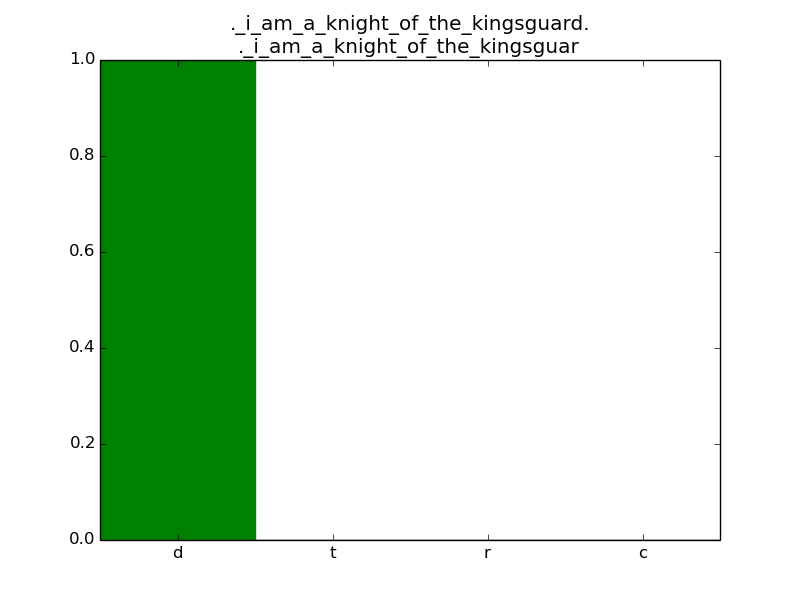
\includegraphics[scale=0.4]{../distplot/31.png}
% \end{center}
% \end{frame}

% \begin{frame}
% \frametitle{Input/Output Example}
% \begin{center}
% 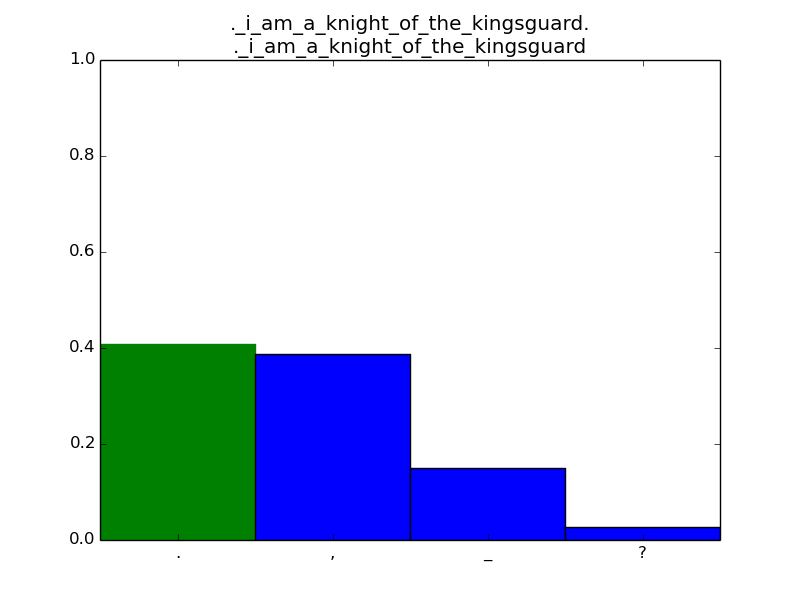
\includegraphics[scale=0.4]{../distplot/32.png}
% \end{center}
% \end{frame}



\section{Not the End}
\begin{frame}
\frametitle{Not yet the End}
\begin{itemize}
\item<1-> Show sample input/output.
\item<1-> Show programs here if there is time.
\end{itemize}
\end{frame}

\end{document}


% title: Text Generation with LSTM Units
% abstract: One of the cool things one can do with neural networks is making them learn from text in an unsupervised manner. The text could be English text, but it could also be any other kind of text, like for example source code. After learning, the neural network should be able to produce new text that is remarkably similar to the text which it learned from. The talk is about a project where this was experimented with.